\begin{figure}
  \centering
  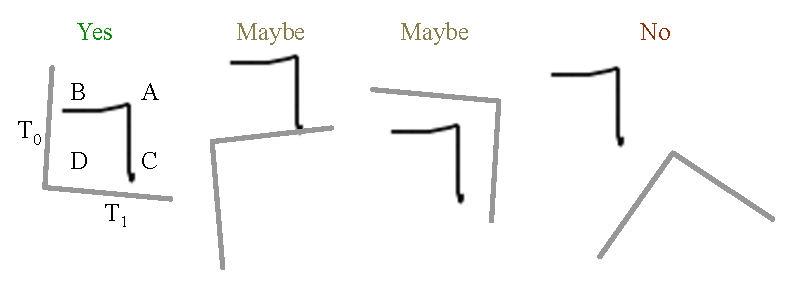
\includegraphics[width=0.9\linewidth]{img/right-angle.pdf}
  \caption[Right Angle]{Context check for Right Angle recognizer. The
    user's input (black) is compared with the position and orientation
    of nearby line segments $T_0$ and $T_1$ (gray) to compute a
    liklihood that the gesture applies to that particular line
    pair. It outputs \textit{Yes}, \textit{Maybe}, or \textit{No}
    depending on how well the context matches the input.}
  \label{fig:right-angle}
\end{figure}
